\section{Where faster serial responses can help}
\label{sec:survives}

\paragraph{Online extraction under a deadline.}
A log processor may need an event's severity and affected component before
deciding whether to request another check. Its response budget covers
queueing, generation, validation, and the decision. A correct record
received too late cannot support that timely action.

\begin{center}
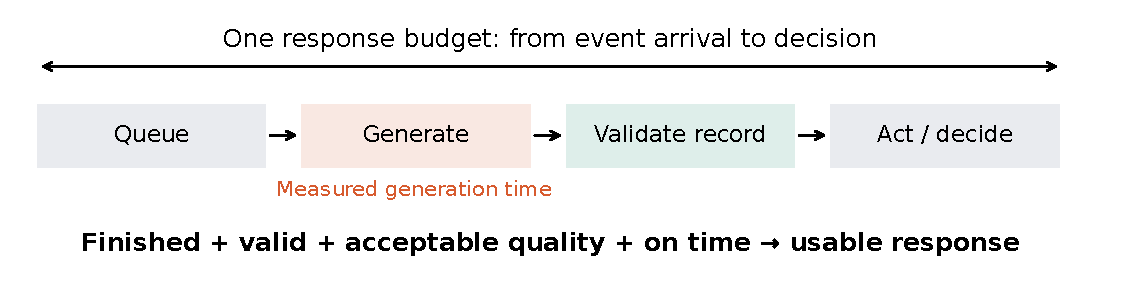
\includegraphics[width=.94\linewidth]{figures/deadline_path.pdf}
\captionof*{figure}{The full response path (schematic). Generation occupies
one stage; the remaining stages also consume the deadline.}
\end{center}

The completion fractions in \S\ref{sec:wins} quantify generation.
They make DG a useful candidate when this stage has a tight budget and
its quality is sufficient. A complete canvas still needs validation;
an on-time error does not become useful just because it arrived quickly.
End-to-end decisions require measurements of the remaining stages.

\paragraph{Dependent investigations and longer responses.}
In an investigation, the next query may depend on an earlier answer.
Such dependencies make per-call latency accumulate, even while other
investigations run concurrently. Lower latency can shorten the time to
the next useful observation. The saved chain experiment supports this
motivation using the smaller AR-3B baseline; it is reported separately
in Appendix~\ref{app:secondary}, not as an AR-30B chain benchmark.

A long response and a chain of responses are different workloads.
The first can spread DG's initial canvas cost over more required tokens;
the second repeats input processing and generation across dependent calls.
Both motivate evaluating diffusion, but neither guarantees a benefit at
arbitrary lengths. Long-form reasoning and repeated code generation also
require suitable quality. The exploratory code results in
Appendix~\ref{app:humaneval} show a substantial quality gap, so they do not
establish successful long investigations for the primary pair.

\paragraph{Choosing the configuration.}
Measure required output length and quality, then check on-time record
validity under the intended arrival rate. Canvas size and refinement effort
change the balance, but truncating an output budget is not the same as
reducing refinement passes. Supporting sweeps document these effects;
the main comparison retains the reference configuration.
